\RequirePackage{fix-cm}
\documentclass[twocolumn]{svjour3}
% DRAFT 2 -- for the second draft discussion (after the full experiment on 424 test dishes).
% Complete paper. Red in brackets = open decision for the discussion.

\usepackage{cite}
\usepackage{graphicx}
\usepackage{amsmath}
\usepackage{amssymb}
\usepackage{xcolor}
\usepackage{booktabs}
\usepackage{multirow}
\usepackage{url}
\usepackage{balance}

\newcommand{\open}[1]{\textcolor{red!70!black}{[#1]}}
\graphicspath{{figs/}}
\setlength{\emergencystretch}{2em}   % fewer overfull lines in two columns
\def\UrlBreaks{\do\/\do-\do.\do\_}

\journalname{Draft 2 -- for discussion}

\begin{document}

\title{Two Questions Are Enough: Budgeted User Questions for Calorie Estimation from Meal Photos}
\titlerunning{Budgeted user questions for photo-based calorie estimation}

\author{Adam~Soko{\l}owski \and Antoni~Grajek}
\authorrunning{A.~Soko{\l}owski, A.~Grajek}

\institute{A.~Soko{\l}owski, A.~Grajek \at
  Warsaw University of Technology, \open{faculty / institute to confirm}
}

\date{Draft 2 (full results)}

\maketitle

\begin{abstract}
Vision-language models can estimate the energy content of a meal from a single photograph, but they cannot
see portion size or hidden fat, and their errors remain large. Interactive systems reduce this error by
asking the user, yet existing work asks many questions and assumes that the user knows the exact answers.
We studied a realistic setting in which an application may ask at most three questions and people answer
with error. On 424 test dishes from Nutrition5k we evaluated an open model, Qwen2.5-VL-7B, with a pool of
seven questions, eight simulated users calibrated on human portion-estimation data and five
question-selection strategies, including a learned selector driven by the model's uncertainty. Two
well-chosen questions lowered the mean absolute percentage error from 52.8\% to 43.9\%, recovering 84\% of
the gain obtained with all seven answers (42.2\%). The learned selector beat random choice and a model that
chose its own questions, but it was not better than a fixed question order. Asking whether the portion was
small, medium or large was the most useful question for every user; noisy answers removed 37\% of the value
of asking for grams, and asking for an ingredient list or about added fat increased the error. For
calorie-tracking applications, a short fixed questionnaire about portion size is therefore a strong and
simple default.
\keywords{calorie estimation \and vision-language models \and clarifying questions \and active feature acquisition \and Nutrition5k}
\end{abstract}

% =====================================================================
\section*{Questions for the second discussion}
\begin{enumerate}
  \item \textbf{Reference for H1.} After the pilot we planned to measure H1 against the oracle. On the full
        test set all seven answers do help, so the original definition works again: 84\% of the gain
        (H1 met) versus 32\% of the oracle's gain (H1 not met). The draft reports the original definition
        first and the oracle share second. Is this acceptable?
  \item \textbf{Framing of the negative result.} The learned selector is not better than a fixed order
        (MAPE). The title and abstract present ``a fixed order is enough'' as a finding. Agreed?
  \item \textbf{Secondary metrics.} For the ideal user the selector has about 6\,kcal lower MAE and 4--6
        points higher acc@20\% than the fixed order, but only one of these differences survives the Holm
        correction. Report it as a secondary observation or leave it out?
  \item \textbf{Pilot versus test.} In the 43-dish pilot all answers increased the error; on 424 test dishes
        they reduced it. Is one sentence in the Limitations enough?
  \item \textbf{Venue and length.} Target journal or conference, page limit, and whether the eight-user
        figure goes to an appendix.
\end{enumerate}

% =====================================================================
\section{Introduction}
\label{sec:intro}

Photo-based food logging is one of the most convenient ways to track energy intake, and general-purpose
vision-language models (VLMs) now make it possible without task-specific training. Their estimates,
however, remain imprecise. On Nutrition5k~\cite{thames2021nutrition5k}, dedicated models reach a calorie
error of 26\% from a single RGB image and 15--19\% with real or predicted
depth~\cite{thames2021nutrition5k,han2023dpf}, whereas zero-shot GPT-4V has a mean absolute percentage
error (MAPE) of 55\%~\cite{tanabe2024calorielava}, and recent commercial models still miss by about 36\%
on standardised photographs~\cite{fridolfsson2025llm}. The gap is not only a matter of model size: the
image itself lacks the information that matters most.

Two sources of error dominate. The first is portion size, because a single overhead photo does not show
the third dimension; volume estimation has long been the weakest stage of image-based dietary
assessment~\cite{lo2020review,vinod2026portion}, and VLMs in particular recognise food volume
poorly~\cite{tanabe2025calorievol}. The second is hidden energy, such as cooking oil, butter and dressings,
which adds many calories while being barely visible~\cite{bhatambarekar2025thesis}. Neither can be fully
recovered from pixels, but both are known to the person who ate the meal.

Asking the user is therefore a natural remedy, and it works. Giving GPT-4o the ingredient masses lowers
its MAPE from about 51\% to 29\%~\cite{bhatambarekar2025thesis}, contextual metadata improves large
multimodal models~\cite{coburn2025lmm}, and an agent that asks its own clarifying questions beats a fixed
question sequence~\cite{bhatambarekar2026agentic}. Not every piece of information is worth asking for,
though: the dish name alone barely changes the error of an image model~\cite{narang2025multimodal}.

Existing interactive work leaves two practical questions open. First, it either asks every question in a
fixed ladder or lets an agent ask without limit, while each extra question adds user burden, and in dietary
assessment lower burden usually comes at the cost of lower accuracy~\cite{hochsmann2020review}. How much
accuracy one, two or three questions can buy, and which questions they should be, has not been measured.
Second, answers are taken from the dataset's ground truth, although people estimate portions poorly: only
35--50\% of their estimates fall within $\pm$25\% of the true mass~\cite{lucassen2021portion}. It is unknown
how much of the reported gain survives realistic answers, and whether the ranking of useful questions
changes. Methods for selecting what to ask under a cost, studied as active feature
acquisition~\cite{aronsson2025afa} and as information-gain-driven clarification for language
models~\cite{kobalczyk2025active,infogain2026clarification}, have not been applied to this problem.

We address these gaps with three research questions. \textbf{RQ1:} how does the calorie error depend on a
question budget of 0--3? \textbf{RQ2:} does an uncertainty-driven, image-dependent question selector
outperform a fixed order, random choice and a VLM choosing its own questions at the same budget?
\textbf{RQ3:} how do noisy and coarse answers change the value of interaction and the ranking of questions?
We test four hypotheses: two well-chosen questions give at least 70\% of the error reduction of full
information (H1); the learned selector is significantly better than random and fixed-order selection and
not worse than the agent (H2); realistic noise reduces the gain of the grams question by at least 30\% and
makes categorical questions competitive (H3); and the fat question helps most for fat-rich dishes (H4).

Our contributions are (1) an evaluation protocol for budgeted interactive calorie estimation with
simulated users calibrated on human data, (2) error-versus-budget curves and a strategy comparison for an
open VLM on Nutrition5k, and (3) evidence on which questions are worth asking real users. The main finding
is that the choice of questions matters more than the cleverness of the selection: two questions about
portion size give most of the gain, and a fixed order is as good as a learned selector.

% =====================================================================
\section{Related work}
\label{sec:related}

\paragraph{Image-based calorie estimation.}
Im2Calories~\cite{meyers2015im2calories} established the recognition--segmentation--volume pipeline and
showed that portion is its hardest stage, a conclusion repeated by later reviews~\cite{lo2020review,vinod2026portion}.
Nutrition5k~\cite{thames2021nutrition5k} provided cafeteria dishes with weighed ingredients and overhead
RGB-D images, and models with predicted depth~\cite{han2023dpf} or richer datasets~\cite{yu2026omnifood8k}
now lead single-image benchmarks. Such models rely on large-scale pre-training that public alternatives do
not match~\cite{andrade2025pretraining}, which makes general-purpose VLMs an attractive alternative.

\paragraph{Multimodal language models for nutrition.}
Fine-tuning LLaVA on Nutrition5k lowers its error below that of GPT-4V~\cite{tanabe2024calorielava}, and
adding an estimated volume to the prompt helps further~\cite{tanabe2025calorievol}. Other systems combine
VLMs with retrieval and conversation~\cite{yao2024caloraify} or with reinforcement-learned
reasoning~\cite{zhu2026foodr1}. Benchmarks of zero-shot models show large errors and a strong dependence on
the model and the prompt~\cite{fridolfsson2025llm,coburn2025lmm,nutrients2026prompt}.

\paragraph{Interaction with the user.}
The closest work evaluates eight multimodal models with a ladder of cues (ingredients, total mass,
ingredient masses) and with an agent that asks its own questions~\cite{bhatambarekar2025thesis,bhatambarekar2026agentic}.
Total mass is the strongest single cue, and agentic questioning beats a fixed sequence. Both studies use
exact answers from the dataset and no question budget; we add both constraints.

\paragraph{Choosing what to ask.}
Active feature acquisition selects, per instance, which features to acquire under a cost; strategies range
from static orders to greedy and reinforcement-learned policies~\cite{aronsson2025afa,schutz2025afabench}.
Language models can supply prior knowledge for this choice, but they plan acquisition sequences
poorly~\cite{perets2026zeroshot}. For clarifying questions, maximising expected information gain improves
task disambiguation~\cite{kobalczyk2025active,infogain2026clarification}, and models rarely ask useful
questions unless trained to do so~\cite{zhang2024clarifying}. We follow the acquisition view and keep the
selector separate from the estimating VLM.

% =====================================================================
\section{Methods}
\label{sec:methods}

Figure~\ref{fig:pipeline} shows the pipeline. For each dish, a strategy chooses up to $B$ questions, a
simulated user answers them, and the VLM estimates the energy from the photo and the answers.

\begin{figure*}[t]
  \centering
  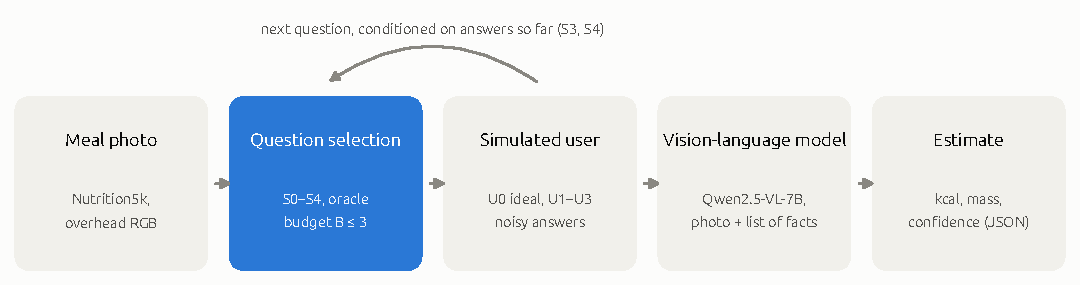
\includegraphics[width=0.9\textwidth]{fig_pipeline}
  \caption{Evaluation pipeline. A strategy selects up to $B\le 3$ questions, a simulated user answers them
  (possibly with error), and the vision-language model estimates energy from the photo and the answers.}
  \label{fig:pipeline}
\end{figure*}

\subsection{Data}
We used Nutrition5k~\cite{thames2021nutrition5k}, which contains real cafeteria dishes with weighed
ingredients and overhead RGB photographs; we downloaded only the overhead images and the metadata. A
validation set of 300 dishes was sampled with a fixed seed from the official training split and used to fit
strategies; the official test split was used for evaluation. A pilot on 50 validation dishes showed that
plates under 50\,kcal dominate the percentage error (seven such dishes raised the photo-only MAPE from 39\%
to 85\%), so we excluded them. The test set then contained 424 dishes with a median of 270\,kcal (range
50--1051) and 197\,g, five ingredients and 42\% of energy from fat on average; 70\% of dishes obtained more
than 30\% of their energy from fat.

\subsection{Question pool}
Table~\ref{tab:questions} lists the seven questions. True answers were derived from the metadata: the fat
and sauce questions use hand-made ingredient lists, and the size categories use the terciles of dish mass on
the validation set ($<$153\,g, 153--288\,g, $>$288\,g), which were shown to the model with the answer.
Answers enter the prompt as an unordered list of facts, so a set of questions defines the prompt
independently of the order in which they were asked.

\begin{table}[t]
  \centering
  \caption{Question pool and the source of the true answer in Nutrition5k.}
  \label{tab:questions}
  \setlength{\tabcolsep}{3pt}
  \begin{tabular}{@{}lp{3.2cm}p{3.1cm}@{}}
    \toprule
    ID & Question & True answer \\
    \midrule
    Q1 & How much did the meal weigh (g)? & total mass \\
    Q2 & Was the portion small, medium or large? & mass tercile \\
    Q3 & Was it fried, or was oil/butter added? & fat ingredient present \\
    Q4 & Was there a sauce or dressing? & sauce ingredient present \\
    Q5 & What is the main ingredient? & heaviest ingredient \\
    Q6 & Please list the ingredients. & ingredient list \\
    Q7 & How many separate items are on the plate? & ingredients $\ge$10\,g \\
    \bottomrule
  \end{tabular}
\end{table}

\subsection{Simulated users}
The ideal user U0 returns the true answers, as in prior work. User U1 perceives mass with a log-normal
error, $m' = m\,e^{\varepsilon}$ with $\varepsilon\sim\mathcal{N}(\mu,\sigma)$; we used $\sigma\in\{0.1, 0.33,
0.5\}$ and a variant with $\sigma=0.33$, $\mu=0.2$ (over-estimation). The value $\sigma=0.33$, our main
realistic user, puts 56\% of answers within $\pm$25\% of the truth, close to the 50\% reported for textual
portion descriptions~\cite{lucassen2021portion}. The size category (Q2) uses the same perceived mass, so the
user is consistent. User U2 makes categorical mistakes with probability $p\in\{0.1, 0.2\}$: an adjacent
size category, a flipped yes/no answer, the second heaviest ingredient, a forgotten ingredient or a count
off by one. User U3 answers ``I don't know'' with probability $q=0.2$, and the question still uses up the
budget. Answers were drawn once per dish and user, so a user gives the same answer whatever else is asked.

\subsection{Model and prompt}
We used Qwen2.5-VL-7B-Instruct in 4-bit AWQ quantisation, served with vLLM on a single 8\,GB laptop GPU.
The prompt contained the photo, the list of facts and a request for a JSON object with energy (kcal), mass
(g) and a confidence between 0 and 1, decoded at temperature 0. In the pilot a short reasoning field before
the numbers made the estimates worse and doubled the time per call, so we used direct JSON output. Because
the prompt depends only on the set of questions, we computed predictions for every subset of size at most
three ($1+7+21+35=64$ subsets) and every user, and evaluated all offline strategies by lookup. For the four
additional sensitivity users ($\sigma=0.1$, $\sigma=0.5$, bias, $p=0.2$) we limited the budget to two. Identical prompts were computed once; the
whole experiment took about 112 thousand model calls and 36 hours. The model returned valid JSON for every
call.

\subsection{Question-selection strategies}
\textbf{S0} uses the photo only. \textbf{S1} chooses questions at random; we report its exact expectation
over all subsets of size $B$. \textbf{S2} asks questions in a fixed order, built greedily on the validation
set to minimise mean error (for U0: Q2, Q5, Q4). \textbf{S3} lets the VLM choose the next question itself
from the remaining pool, step by step, given the answers so far; it was run for U0 and the main noisy user,
and 1.6\% of its choices were invalid and replaced by the first remaining question. \textbf{S4}, our
selector, is a gradient-boosted regressor (LightGBM) that predicts, for each candidate question, the
reduction in the dish's absolute percentage error when that question is added. Its features describe the
model's uncertainty (spread of $K=5$ photo-only samples at temperature 0.7, stated confidence), the current
and photo-only estimates, the answers obtained so far and the user's noise parameters; it was trained on
the validation set, pooled over users. S4 picks the question with the largest predicted gain, greedily,
until the budget is used. The \textbf{oracle} chooses, with knowledge of the true energy, the best subset of
size at most $B$ for each dish, including asking nothing, and is an upper bound that no real strategy can
reach.

\subsection{Metrics and statistics}
The main metric is MAPE; we also report MAE (kcal) and the share of estimates within $\pm$20\% of the truth
(acc@20\%). For H1 we report the gain a strategy recovers relative to asking all seven questions,
$(\mathrm{MAPE}_{S0}-\mathrm{MAPE}_{s})/(\mathrm{MAPE}_{S0}-\mathrm{MAPE}_{\mathrm{all}})$, and its share of the
oracle's gain at the same budget. Strategies are compared with the paired Wilcoxon signed-rank test on
per-dish errors, with bootstrap 95\% confidence intervals (2000 resamples) of the mean difference and Holm
correction within each user; acc@20\% is compared with the exact McNemar test.

% =====================================================================
\section{Results}
\label{sec:results}

\subsection{Error versus number of questions}
With the photo only, the model had a MAPE of 52.8\% on the test set (MAE 121\,kcal, 26\% of dishes within
$\pm$20\%). All seven answers of the ideal user lowered it to 42.2\% (Table~\ref{tab:main},
Fig.~\ref{fig:budget}). Most of this gain came from the first two questions: with S4, one question gave
47.7\%, two 43.9\% and three 42.7\%. Two questions therefore recovered 84\% of the gain of full information
(S2: 82\%), above the 70\% threshold of H1. The oracle reached 24.6\% at $B=2$, so S4 obtained 32\% of the
oracle's gain at the same budget.

\begin{figure*}[t]
  \centering
  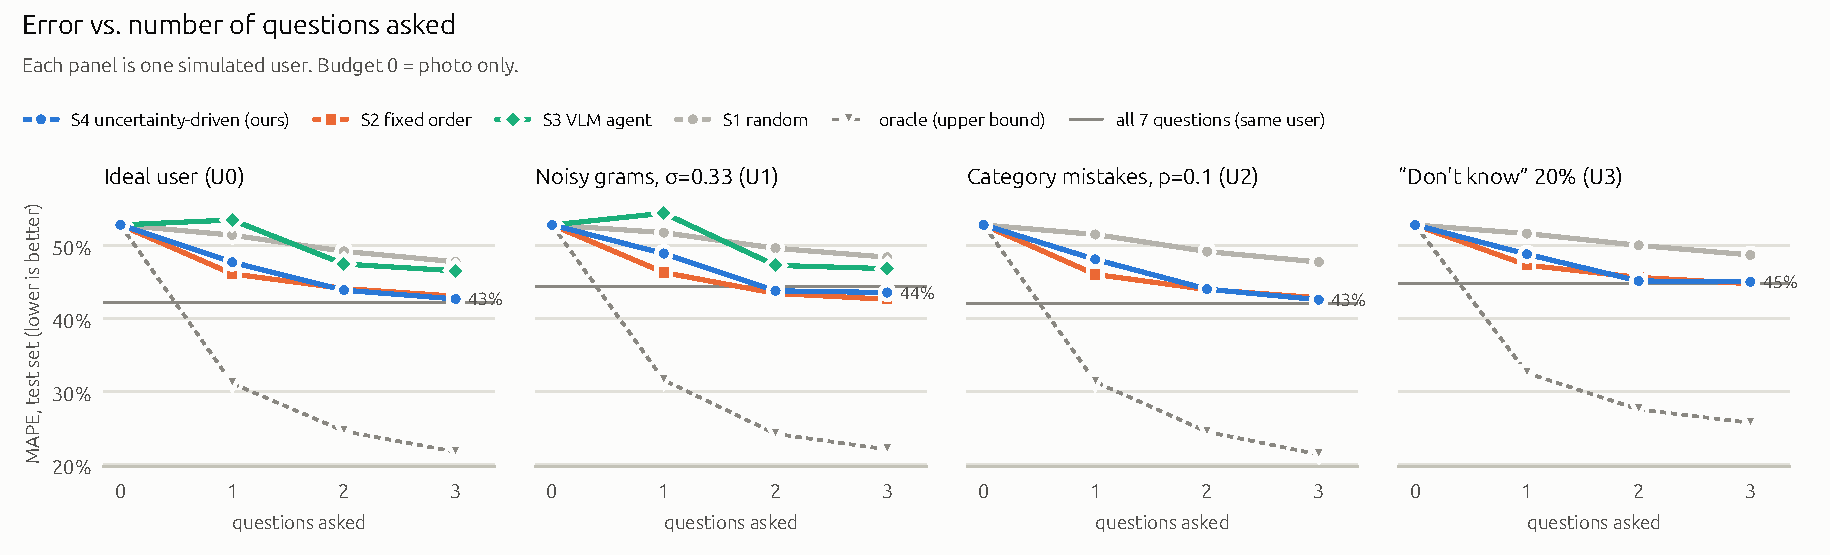
\includegraphics[width=\textwidth]{fig1_budget_curves}
  \caption{Calorie error (MAPE, test set, $n=424$) versus the number of questions asked, for four simulated
  users. Budget 0 is the photo only; the horizontal line is the error with all seven questions.}
  \label{fig:budget}
\end{figure*}

\begin{table}[t]
  \centering
  \caption{MAPE [\%] on the test set ($n=424$). Photo only: 52.8\%. All seven questions: 42.2\% (U0),
  44.4\% (U1, $\sigma=0.33$).}
  \label{tab:main}
  \setlength{\tabcolsep}{3.5pt}
  \begin{tabular}{@{}llrrrrr@{}}
    \toprule
    User & $B$ & S1 & S2 & S3 & S4 & Oracle \\
    \midrule
    \multirow{3}{*}{U0 ideal}           & 1 & 51.4 & 46.1 & 53.5 & 47.7 & 31.1 \\
                                        & 2 & 49.2 & 44.1 & 47.5 & 43.9 & 24.6 \\
                                        & 3 & 47.8 & 43.1 & 46.5 & 42.7 & 21.7 \\
    \midrule
    \multirow{3}{*}{U1 $\sigma{=}0.33$} & 1 & 51.8 & 46.3 & 54.5 & 48.9 & 31.6 \\
                                        & 2 & 49.6 & 43.5 & 47.3 & 43.8 & 24.2 \\
                                        & 3 & 48.4 & 42.6 & 46.8 & 43.6 & 22.0 \\
    \bottomrule
  \end{tabular}
\end{table}

\subsection{Comparison of strategies}
S4 had a significantly lower error than random selection for every user at $B=1$ and $B=2$ (all
$p_{\text{Holm}}\le 0.03$) and lower than the VLM agent for both users on which the agent was run
(Table~\ref{tab:tests}). It was not significantly different from the fixed order: the mean differences
ranged from $-2.5$ to $+2.6$ percentage points across users and budgets, and every confidence interval
contained zero. H2 is therefore only partly supported. The agent was the weakest strategy at $B=1$, worse
than the photo alone (53.5\% versus 52.8\%); it asked for the portion size for 47\% of dishes, for the
ingredient list for 36\% and for the number of items for 15\%.

On secondary metrics S4 tended to be better than S2 for the ideal user: its MAE was 6\,kcal lower at every
budget (raw $p=0.02$--$0.05$) and its acc@20\% 4--6 points higher, but after Holm correction only the
acc@20\% difference at $B=3$ remained significant (33.0\% versus 27.6\%, $p_{\text{Holm}}=0.04$). For noisy
users there was no consistent difference.

\begin{table}[t]
  \centering
  \caption{Paired comparison of S4 with other strategies: mean difference in MAPE [pp] (negative = S4
  better), bootstrap 95\% CI and Holm-adjusted Wilcoxon $p$.}
  \label{tab:tests}
  \setlength{\tabcolsep}{2.6pt}
  \begin{tabular}{@{}llrrr@{}}
    \toprule
    User, $B$ & vs & $\Delta$ & 95\% CI & $p_{\text{Holm}}$ \\
    \midrule
    \multirow{3}{*}{U0, 1} & S1 & $-3.7$ & $[-6.4, -1.0]$ & 0.002 \\
                           & S2 & $+1.6$ & $[-1.9, +5.4]$ & 0.590 \\
                           & S3 & $-5.8$ & $[-10.3, -1.5]$ & 0.007 \\
    \midrule
    \multirow{3}{*}{U0, 2} & S1 & $-5.3$ & $[-7.7, -3.0]$ & $<$0.001 \\
                           & S2 & $-0.2$ & $[-3.2, +3.0]$ & 0.276 \\
                           & S3 & $-3.6$ & $[-6.6, -0.3]$ & 0.002 \\
    \midrule
    \multirow{3}{*}{U1, 1} & S1 & $-2.9$ & $[-5.3, -0.4]$ & 0.013 \\
                           & S2 & $+2.6$ & $[-0.7, +6.2]$ & 0.815 \\
                           & S3 & $-5.5$ & $[-9.9, -1.3]$ & 0.026 \\
    \midrule
    \multirow{3}{*}{U1, 2} & S1 & $-5.8$ & $[-8.3, -3.4]$ & $<$0.001 \\
                           & S2 & $+0.4$ & $[-2.7, +3.7]$ & 0.815 \\
                           & S3 & $-3.5$ & $[-7.0, +0.1]$ & 0.038 \\
    \bottomrule
  \end{tabular}
\end{table}

\subsection{Noisy answers and the ranking of questions}
Noise lowered the value of interaction but did not change its shape (Fig.~\ref{fig:budget}): with the main
noisy user ($\sigma=0.33$) two questions still gave 43.8\% with S4 and 43.5\% with S2, and all seven answers
44.4\%. Asked alone, the grams question (Q1) reduced the error by 5.9 points for the ideal user and by 3.7
points for the noisy one, a drop of 37\%, above the 30\% threshold of H3 (Fig.~\ref{fig:ranking}). The size
category (Q2) was then more useful than grams (6.5 points). It was, however, already the most useful
question for the ideal user, so the ranking did not change: Q2, Q1, Q4, Q7, Q5, Q3, Q6 for both users. H3 is
therefore partly supported. The ingredient list (Q6) increased the error by about 7 points for every user,
and the fat question (Q3) did not help on average ($-0.4$ points).

\begin{figure*}[t]
  \centering
  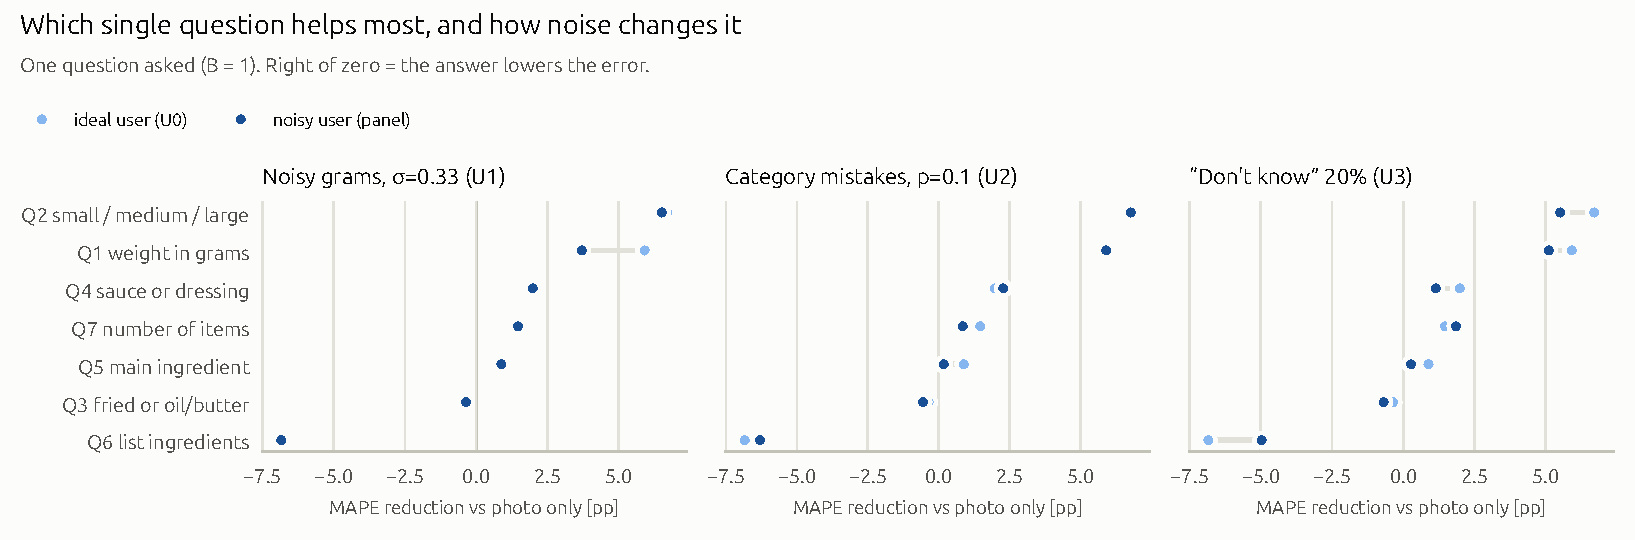
\includegraphics[width=\textwidth]{fig2_question_ranking}
  \caption{Change in MAPE when a single question is asked (positive = lower error), for the ideal user
  (light) and three noisy users (dark).}
  \label{fig:ranking}
\end{figure*}

\subsection{Subgroups}
For fat-rich dishes (more than 30\% of energy from fat, $n=297$), the fat question increased the error by
3.2 points, and the size category was the most useful question (5.6 points; Fig.~\ref{fig:subgroups}). The
fat question helped only the leaner dishes (6.2 points), so H4 is not supported. The size category reduced
the error by 20.6 points for small portions and did not help large ones.

\begin{figure}[t]
  \centering
  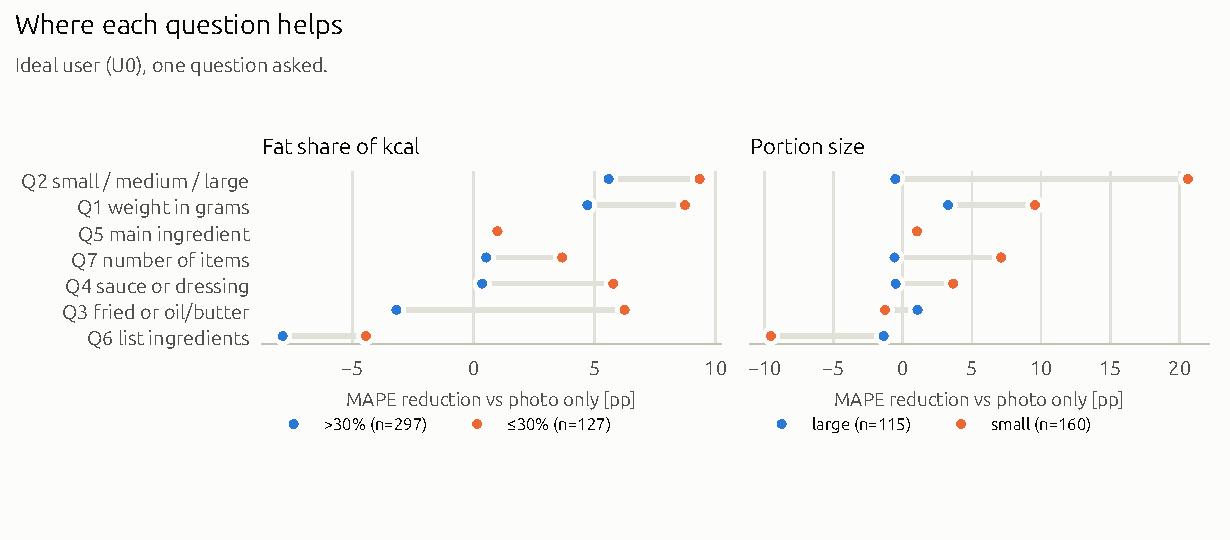
\includegraphics[width=\columnwidth]{fig3_subgroups_U0}
  \caption{Single-question gain in subgroups (ideal user): share of energy from fat and portion size.}
  \label{fig:subgroups}
\end{figure}

\subsection{Per-dish headroom and the direction of errors}
The oracle's advantage comes from choices that differ between dishes. For the ideal user, the best single
question was the grams question for 53\% of dishes and the size category for 27\%, the first question of
the fixed order. For 45\% of dishes no single question lowered the error at all, so a strategy that could
also decide not to ask would gain on these dishes. The model's photo-only errors were not uniform in sign:
it over-estimated on average (mean signed error $+21\%$, median $+5\%$). The ingredient list increased this
bias to $+37\%$ (median $+20\%$), the fat question slightly ($+25\%$), and the size category reduced it
($+14\%$, median $+2\%$). Sampling the model five times at temperature 0.7 gave identical estimates for 95\%
of dishes, so the spread of samples carried almost no information about the error.

% =====================================================================
\section{Discussion}
\label{sec:discussion}

The answer to RQ1 is that two questions are enough. Two well-chosen questions recovered 84\% of the error
reduction of all seven, and the third added about one percentage point. This agrees with the strong value of
total mass reported for larger models~\cite{bhatambarekar2025thesis}, but here the most useful single cue
was the coarse size category rather than the exact mass, which matters for applications because a category
is easier for people to give. Diminishing returns after two questions also mean that the user's burden can
be kept low without a large loss of accuracy~\cite{hochsmann2020review}.

For RQ2, the learned selector did not beat a fixed order, although it beat random choice and the VLM's
own choices. The most likely reason is that the uncertainty signal it was built on barely exists for this
model: the sampled estimates were identical for 95\% of dishes, so the selector had little to condition on,
and its most important features were the candidate question and the current estimate. The agent's poor
first choices (often the ingredient list) agree with the observation that language models plan information
acquisition poorly~\cite{perets2026zeroshot} and rarely ask useful questions without training for
it~\cite{zhang2024clarifying}; they contrast with the advantage of agentic questioning reported for larger
proprietary models~\cite{bhatambarekar2026agentic}. At the same time the oracle shows substantial headroom:
choosing the right question for each dish, or not asking at all, would roughly halve the error. Better
uncertainty estimates, for example from paraphrased prompts or token probabilities, are the natural way to
exploit it, in the spirit of information-gain-driven
clarification~\cite{kobalczyk2025active,infogain2026clarification}.

For RQ3, realistic noise removed more than a third of the value of the grams question but changed
neither the shape of the budget curves nor the ranking of questions, because the categorical size question
was already the most useful one. Two questions hurt: the ingredient list and, for fat-rich dishes, the fat
question. Both pushed an already over-estimating model further up. A plausible mechanism is that the model
adds energy for every mentioned item or for the word ``oil'' instead of updating its estimate of the
portion. This contradicts our expectation (H4) and shows that the value of a question depends on how the
model uses the answer, not only on how informative the answer is.

These results suggest a simple recommendation for calorie-tracking applications built on an open VLM: ask
whether the portion was small, medium or large, then for the main ingredient, and avoid asking for grams
or ingredient lists. A learned, per-image selector is only worth its complexity if the model provides a
usable uncertainty signal.

\paragraph{Limitations.}
We evaluated one 7B model in 4-bit quantisation; larger or proprietary models may use facts differently.
Users were simulated with noise models calibrated on literature rather than on our own study. Nutrition5k
contains cafeteria food from one source, photographed from above. MAPE is sensitive to small dishes, which
we addressed by excluding plates under 50\,kcal. In the 43-dish pilot all answers together increased the
error, while on the 424 test dishes they reduced it; small evaluation sets are therefore unreliable for this
task.

\paragraph{Future work.}
A second VLM of another family, a study with real users answering questions about Nutrition5k photos, and
selectors that use better uncertainty estimates and can decide not to ask.

% =====================================================================
\section{Conclusions}
\label{sec:conclusions}
Under a budget of up to three questions, two questions recovered most of the error reduction that all seven
answers provide, both for ideal and for noisy users. A fixed question order was as accurate as a learned,
uncertainty-driven selector and better than letting the model choose its own questions. The size category
was the most useful question for every simulated user, grams lost a third of their value under realistic
noise, and an ingredient list or a question about added fat increased the error. A short fixed questionnaire
about portion size is therefore a strong default, and per-dish question selection remains a promising
direction once models provide reliable uncertainty.

\section*{Statements and Declarations}
The authors declare that no funds, grants, or other support were received during the preparation of this
manuscript. The authors have no relevant financial or non-financial interests to disclose. Code and results
are available at \url{https://github.com/Qasdfyk/how-many-questions}.

\balance
\bibliographystyle{spmpsci}
\bibliography{references}

\end{document}
